
%%%%%%%%% PROPOSAL -- 15 pages (including Prior NSF Support)

\section*{\Large Organizational Responsiveness to Open Outside Input:  A Modeling Approach based on Statistical Text and Network Analysis}


% From the NSF Grants Proposal Guide:
% "The Project Description should provide a clear statement of the work
% to be undertaken and must include: objectives for the period of the proposed
% work and expected significance; relation to longer-term goals of the PI's
% project; and relation to the present state of knowledge in the field,
% to work in progress by the PI under other support and to work in progress
% elsewhere."

\section{Introduction}

Nearly every organization strives to respond in a timely and accurate manner to the needs and demands of some external constituency. Firms respond to customers, governments respond to citizens and educational institutions respond to students. The rapid advancement in communications technology over the last two decades has forever transformed the nature, volume and sources of input and feedback available to organizations. In addition, electronic communications have drastically improved the ability of organizations to document and communicate their internal developments. These complimentary developments have ushered into governance what has been termed 'we government' \cite{Linders2012}. Most elected officials can be directly contacted electronically through simple internet tools. Citizens can advertise and sign petitions on the web and attend internet 'town meetings' with their representatives. Regarding the internal activities of government, citizens can access electronic communications of their officials through public records requests, access meeting minutes on the web and, e.g., watch the floor activities of the US House of Representatives on HouseLive.gov. The emerging field of computational social science seeks to address the most pressing social scientific problems through the development of computational and statistical methods that are ideally tailored to the research task at hand. We propose to develop machine learning methods that are precisely tailored to modeling the {\em complete} input, deliberation, policy formation and implementation cycle documented in the electronic record surrounding an organization. Critically, the models we develop will jointly represent the content of relevant streams of text (i.e., topics) and the socio-organizational structure surrounding text generation (i.e., networks). In this collaborative project, which brings together researchers from computer science and political science, we will develop novel methods and apply them to the analysis of government responsiveness to public input across many US county and city governments.


In this project we will develop and apply novel quantitative methods for identifying the cycle of input, response and feedback that leaves its fingerprint on the electronic communications record. We will focus on the nexus between government organizations and their constituents, but the methods we develop will be portable to other types of organizations. Government responsiveness to citizen input offers an ideal venue within which to model the relationship between streams of textual records embedded in different socio-organizational structural contexts (e.g., activist messages sent from independent citizens and regulations produced by a legislative body).  First, in democratic societies there is a common expectation that the government will respond to public demands. Second, the input mode on which we will focus-- direct email from the public to government officials -- is regularly central to government efforts to encourage direct input to the policy creation and implementation processes. Third, and perhaps of greatest practical importance, due to the scope of freedom of information laws in the US, we as researchers can access the public input and internal communications data associated with a multitude of government organizations.




We frame this project by associating different phases in the cycle of governance with four different types of textual streams and sociopolitical organizational contexts: public input (e.g., emails from citizens to government officials, informal internal communications (e.g., emails among officials), formal deliberations (e.g., legislative meeting minutes) and policy outputs (e.g., regulations, laws). We seek to understand these textual themes through the lens of multi-scale multi-corpora dynamic Bayesian latent variable models of textual content (i.e., topics \cite{Blei2003}) and organizational structural contexts (i.e., networks). We will develop (1) several domain-specific models of dynamic content and structure that are tailored to the unique characteristics of each corpus and (2) develop a flexible framework for constructing multi-corpora dynamic models that tie the individual domains together in a modular, extensible manner. The result will be an analytical approach that permits an organization to distill and investigate the dynamics of input, responsiveness and feedback through a common framework of statistical text analysis.  The methods we develop will offer answers regarding several pertinent questions about organizational management of outside input, e.g., is organizational attention to a topic proportional to its attention in outside input, how does an organization adapt to the rise of issues that are novel relative to its current foci, is responsiveness timely?

\begin{wrapfigure}{r}{.5\textwidth}
\vspace{-.5cm}
\begin{center}
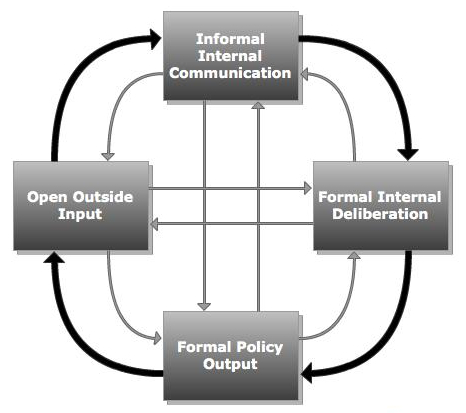
\includegraphics[scale=.525]{cycle.jpg}
\end{center}
\vspace{-.5cm}
\caption{Cycle of input, response and feedback. Black lines denote the normal IRF process and the gray lines represent alternative connections between domains. Direction of arrow indicates the temporal ordering of issue migration.}
\label{cycle}
\end{wrapfigure}

Statistical topic models automatically infer groups of semantically-related words, known as topics, from word co-occurrence patterns within documents. A single topic is characterized by a discrete distribution over some vocabulary. Thus every word in the vocabulary is associated with every topic, albeit with varying probabilities. Given a corpus of documents, statistical topic models simultaneously infer the composition of the topics that best describe that corpus, as well a document-specific distribution over these set of topics for each document. In this way, every document is probabilistically associated with every topic.  \cite{Blei2010}. Statistical topic models provide a dually qualitative and quantitative inferential summary of textual corpora. They are qualitative in that the textual content of a corpus is maintained and quantitative in that the summary of the content is built through large-scale quantitative analysis of patterns in the content.  Since the seminal work on statistical topic models \cite{Blei2003}, the basic framework has been extended and adapted to focus on several aspects of textual corpora; including author-specific distributions over shared topics \cite{Steyvers2004}, dyadic (i.e., author-recipient) aspects of messages \cite{McCallum2005}, the underlying communication network \cite{Krafft2012}, and joint text-metadata models of documents \cite{Mimno2008}. Dynamic topic models \cite{Blei2006} provide an excellent framework within which to understand input to, output from and feedback to organizations that document their activities at various stages in a textual format . In the current project, we propose to develop new Bayesian latent variable models that draw upon the now robust framework of specifying complex topic models that represent textual content of corpora and contextual structure surrounding the generation of the text. This ambitious agenda will involve jointly modeling separate streams of text that influence each other, are informed by rich meta-data, incorporate the underlying communication network, and characterize the over-time aspect of the text streams.


%The benefit from connecting these innovations in statistical topic modeling is that we will leverage a medium common to each domain relevant to a cycle of organizational feedback and responsiveness - textual documentation to connect the domains as well as domain-specific metadata types. For example, in the case of governance, we will tie together the identities of citizens and groups providing outside input, the structure of communication networks underlying informal communications within government and voting coalition patterns within legislatures; all through the medium of the co-evolving, domain-specific text streams.


Figure \ref{cycle} illustrates the cycle of organizational responsiveness that we intend to model through the guise of co-evolving textual streams. Considering the case of governance, substantial research exists that focuses on parts of this cycle. For example, a large body of research exists that documents recent developments in tools for citizens to provide precise, timely and voluminous input to government officials  \cite{Yildiz2007}. There is also a large body of research focusing on legislative adaptation to broad ideological trends among constituents \cite{Canes-Wrone2002}.  And yet another literature that addresses the processes by which topics rise from informal awareness among officials and outside parties to the legislative agenda \cite{Baumgartner1993}. However, due to the historical inaccessibility of timely and common data modes related to each component of the governance cycle, little research has endeavored to connect all of the dots in a data-driven, mathematically principled manner. We will provide such a complete picture, leveraging the common, available, and timely mode of text streams.


In this project we will develop and apply a framework for deriving a complete, multivariate, and interdependent model of external input, internal deliberation and organizational response. Considering government organizations, substantial research has focused on the relationship between public opinion and legislative output  \cite{Canes-Wrone2002,Levendusky2008}, and yet another literature has focused on modeling the relationships between bureaucratic agencies and the legislative agenda \cite{Wood1991,Furlong1998}. However, little -- indeed, as far as we are aware, no -- research has endeavored to build a complete model of the democratic process. The disadvantage of analyzing relationships between domains in a separate, pairwise manner is that it is impossible to reconstruct a complete picture of the cycle of input, response and feedback relevant to an organization.  For instance, in the example of governance, analysis of public input and any one government domain could provide a misleading account of government responsiveness. It may be the case that legislative meeting minutes document consideration of issues that are the subject of considerable public input. However, if final legislation is not responsive, it is not the case that democratic representation has run its complete course. And, initial research indicates that even the most advanced designs for encouraging direct input (i.e., e-petitions that trigger mandatory legislative attention) may end up having little to no policy influence \cite{Hough2012}.

The advantage of our approach will be that we will tap multi-channel input and response processes. This will allow us to identify fast-tracks and bottlenecks in the representation cycle. Identifying the dynamics of the entire system would inform those interested in providing outside input, those seeking to understand the overall responsiveness of an organization and those interested in affecting the organization's responsiveness.



\section{Open Outside Input and Governance}

At every level of government in the US, substantial resources have been dedicated to developing online platforms for citizen input to government. E-Rulemaking \cite{Coglianese2004} -- the process by which proposed regulations are posted to the internet and publicly deliberated on the web -- is the archetype of these efforts. US Federal agencies are required to post proposed rules to the website \texttt{regulations.gov} and provide a period for open commenting on the proposed regulation. Another mainstay of government operations in the information age is online tools to provide direct messages to public officials \cite{Balla2007}. Another recent example of open outside input was provided by President (elect) Obama in 2008. He established \texttt{Change.gov} during the transition to provide for direct citizen input to the administration's future priorities and activities \cite{Borins2009}. These developments mark a potential for rapid, massive and innovative ''citizen-sourcing'' of public policy - a form of democratic representation that is much more timely and rich than that realized through periodic elections and other forms of slower, less interactive input  \cite{Linders2012}.

{\bf Open questions regarding open input:} These developments, which utilize information technology to build a direct bridge between policymakers and their constituents raise several critical questions about their utility. We will develop and apply novel quantitative methods that answer questions such as these:
\begin{itemize}
\item Do the actions of public officials and, ultimately, the content of public policy, reflect the inputs provided by citizens?
\item Do public officials have the capacity to organize and summarize outside inputs?
\item What characteristics of outside input predict the timely integration into public policy?
\end{itemize} All of these questions are critical to determining the value of these e-government or 'we-government' technologies.


We endeavor to answer these questions and more. Using fine-grained textual and contextual data on several stages of the input-response-feedback cycle, we will assess the dynamics of government responsiveness to open outside input on public policy. This will be made possible through the development of machine learning tools that connect multiple textual streams and a massive database of US county government records assembled through public records requests. This project is headed by a multidisciplinary team, which has already realized success in developing innovative machine learning tools to analyze novel databases on government communication networks. We have successfully gathered and processed one-month archives of government officials' in and out-box contents from North Carolina counties including New Hanover, McDowell, Transylvania, Columbus and Moore. With dedicated resources, we are confident we would collect additional data from each county and expand coverage to most of the 100 counties in North Carolina.


\section{Background: Public Records Data}

At the national, state and local levels, the US is the global leader in the scope and reliability of laws that guarantee access to information on government \cite{Halstuk2006}. The seminal legislation in this area is the federal Freedom of Information Act, which marks all information produced by executive agencies as public, unless the information meets at least one of seven criteria for exemption. Most US states have laws that mimic the federal legislation \cite{Braverman1980}, and most state laws subject localities (i.e, cities and counties) to public records archiving and disclosure requirements. North Carolina offers one of the broadest laws. For instance, email communications among local government officials are established by statute to be public record.

Public record disclosure requirements establish a treasure trove for researchers. Many government organizations post significant text streams - from email communications with elected officials to meeting minutes - directly on websites. For categories of information not posted to the web, it is possible to make requests for the data. At all stages of the democratic process, local governments are required to archive textual records and provide them to the public upon request. This constitutes the primary advantage for focusing on government organizations in developing multi-stream models of the input-response-feedback cycle.

For most localities, legislative proceedings and legislative output are available on the city and county websites. Archives of external emails sent to government officials and internal emails are typically not posted on websites, though some counties and cities do indeed post them all. The single data source that we plan to use in this project, which requires government officials' compliance with public records requests is government email. We have had considerable success in gathering email corpora via public records requests for our pilot research (described below). For the pilot data collection, we focused on county governments in North Carolina. The counties whic


\section{Project Team}

The PIs in this project are global leaders in the emerging field of computational social science with substantial publication records in their respective disciplines of computer science and political science, as well as a robust collaborative agenda. The research will be lead by a computer scientist (Wallach) with background in developing machine learning methods for the statistical analysis of text and networks and a political scientist (Desmarais) with background in developing large scale statistical and network analytic models of political decision-making within US government institutions. The team is part of the UMass Amherst Computational Social Science Initiative and has already successfully completed and published pilot research that is highly relevant to the proposed project. This project will combine large-scale data collection, innovative methods development and social scientific analysis, resulting in the following contributions. These innovations will not only appeal to an audience of interdisciplinary scholars in computational social science, but will also constitute important central advancements in computer science and political science.

\begin{itemize}
\item {\bf Central computer science contributions:} Offering substantial contributions to the field of machine learning, we will develop novel Bayesian latent variable models capable of characterizing the relationships between topics in separate dynamic corpora and the socio-organizational contexts within which the text was generated. The contributions offered by these innovations will be of two types: (1) domain-specific dynamic Bayesian latent variable models of textual content and socio-organizational context and (2) the development and implementation of a flexible and extensible approach to building models that represent dynamic interdependence across corpora. These methods will provide a comprehensive textual and contextual data modeling framework that captures cross-domain migration of topics.
\item {\bf Central social science contributions:} We will provide a first-of-its kind, exhaustive micro-level assessment of the function of  democratic representation at the local level. The research we have on democratic responsiveness in the US focuses mainly on the federal or state governments. Our research will address local politics. Also, existing research on democratic representation addresses highly aggregated measures: e.g., showing that legislators from highly conservative districts vote, on average, more conservatively than those from more liberal districts. Our work will provide a fine-grained characterization of government responsiveness to the rise of public demands for action on specific public policy topics.
\end{itemize}



\section{Description of Pilot Research}

As an initial phase of research for this project, we endeavored to leverage our expertise in the computational and social sciences, as well as the availability of rich data sources through the public record to address a challenge in the study of communication networks. this work has been presented at
a variety of computational social science workshops---including the Workshop on Information in Networks, New Directions in Analyzing Text as Data, and the Annual Political Networks Conference---and appeared at Neural Information Processing Systems conference (one of the top machine learning conferences) in late 2012. A substantial body of research finds that the structure of a communication network has a substantial influence on the problem-solving abilities of the network as a whole and the performance of the individuals in the network \cite{Mason2012}. Moreover, recent research indicates that the topic or context of communication is important, meaning the measurement of a communication network should involve topic-of-discussion specificity \cite{Mason2008}. Thus, in order for an organization to diagnose and design its internal communication network, it must first be able to discern topic-specific communication networks.

\begin{figure*}[t]
\begin{minipage}[b]{0.5\linewidth}
\centering
\begin{tabular}{cc}
{\bf Public Signage} &
{\bf Broadcast Messages}\\
{\small change signs sign process ordinance}  &
{\small fw fyi bulletin summary week legislative} \\
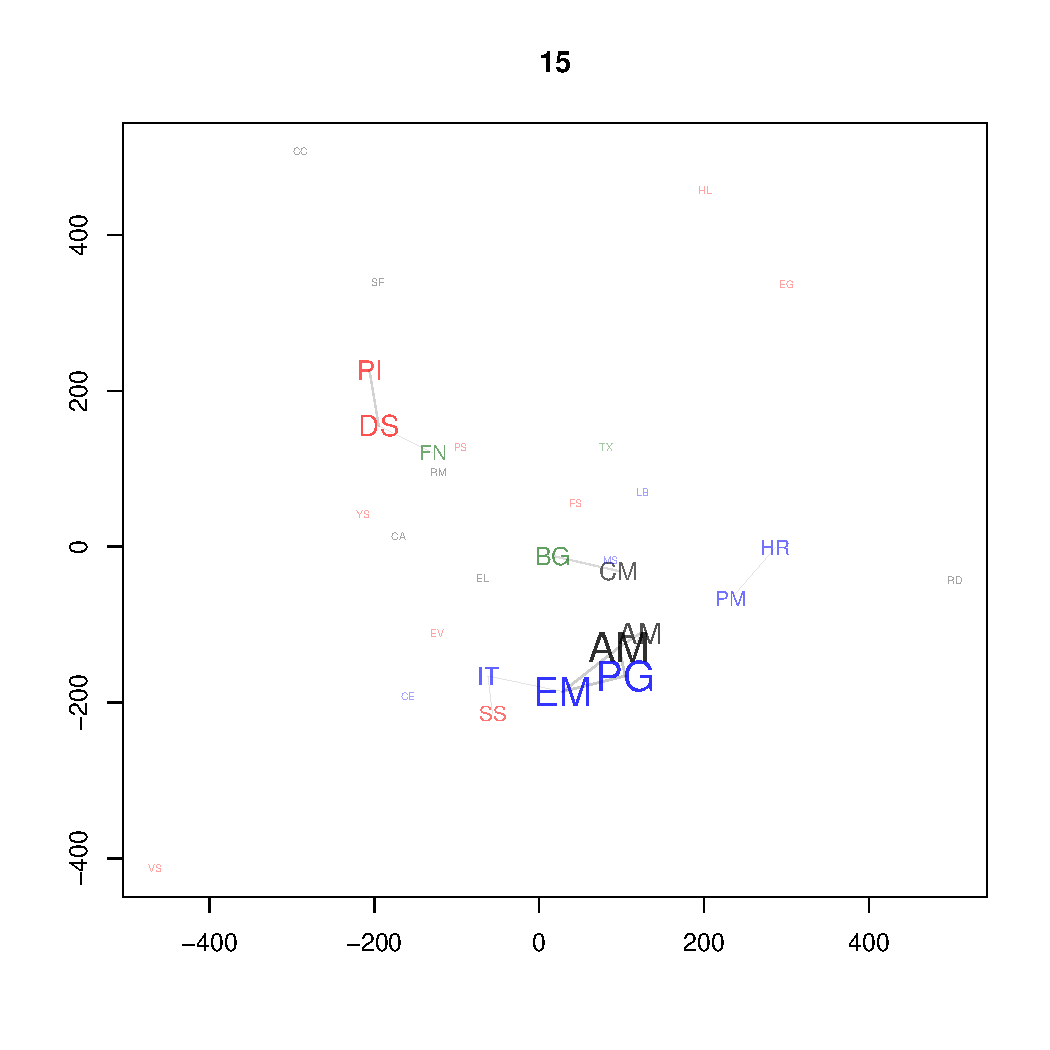
\includegraphics[scale=.29, trim=.4in .6in .4in .8in, clip=true]{latent_space_15} &
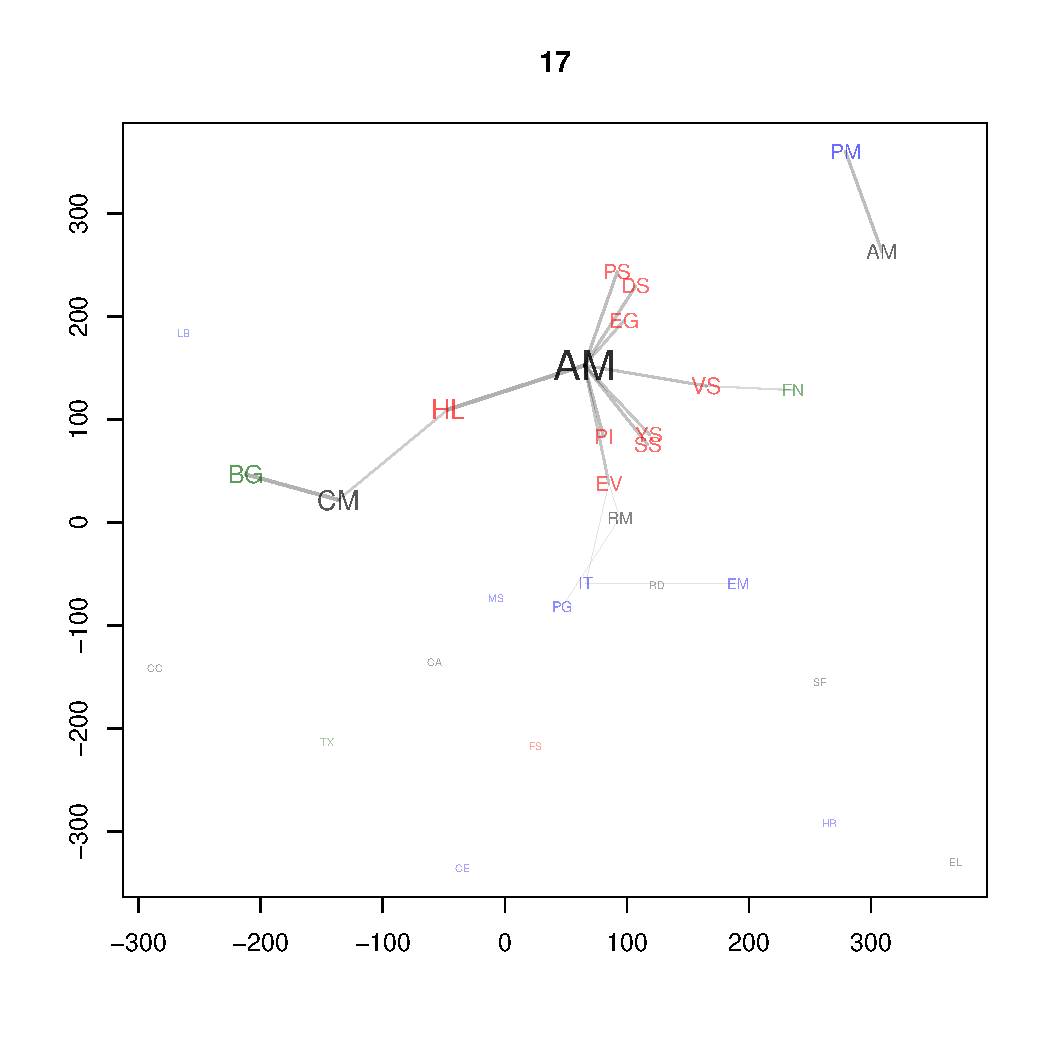
\includegraphics[scale=.29, trim=.4in .6in .4in .8in, clip=true]{latent_space_17} \\
{\bf Public Relations} &
{\bf Meeting Scheduling} \\
{\small city breakdown information give} &
{\small meeting march board agenda week} \\
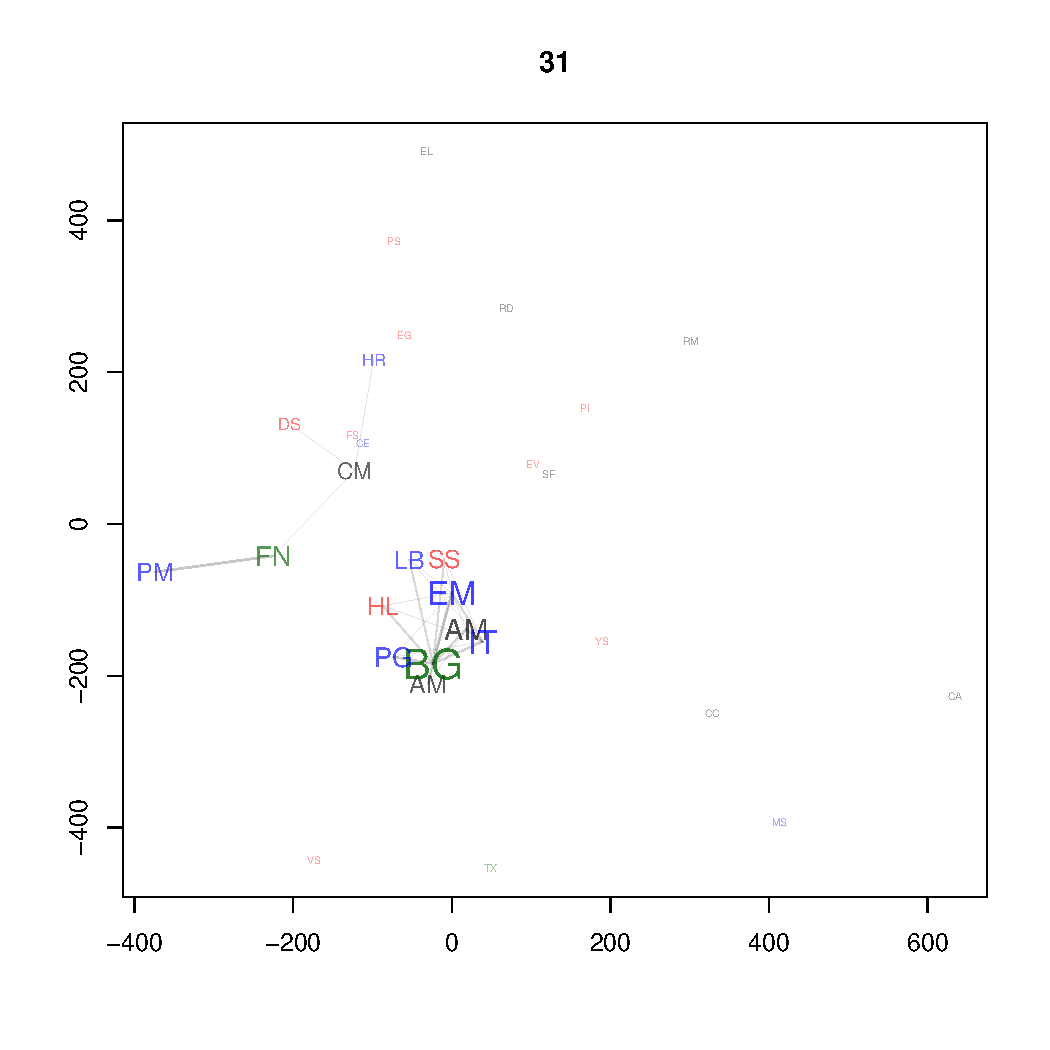
\includegraphics[scale=.29, trim=.4in .6in .4in .8in, clip=true]{latent_space_31} &
 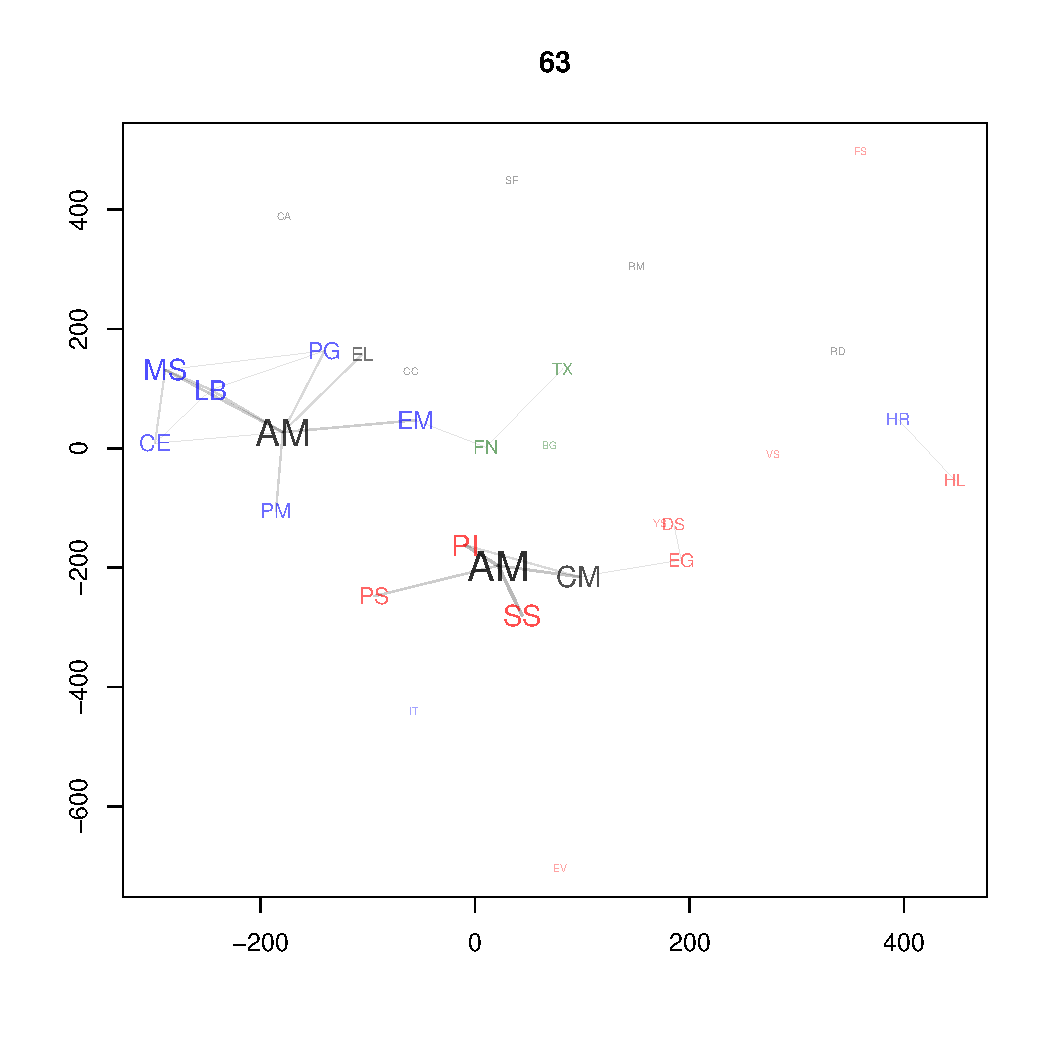
\includegraphics[scale=.29, trim=.4in .6in .4in .8in, clip=true]{latent_space_63} \\
\end{tabular}
\end{minipage}
\begin{minipage}{0.5\linewidth}
\hspace{3.25cm}\vspace{-0.4cm} 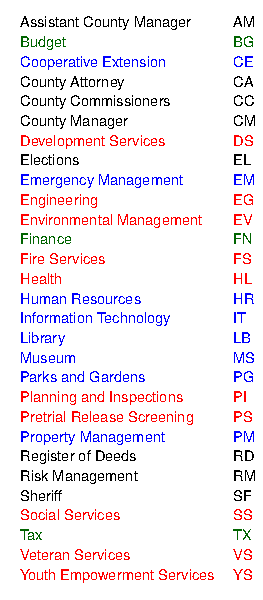
\includegraphics[scale=.85]{department_key}
\end{minipage}
\caption{Four topic-specific communication patterns inferred from the
  NHC email network. Each pattern is labeled with a human-selected
  name for the corresponding topic, along with that topic's most
  probable words in order of decreasing probability. The size of each
  manager's acronym in topic $t$'s pattern (given by $0.45 +
  1.25\,\sqrt{d^{(t)}_a \,/\, \max_a d^{(t)}_a}$, where $d^{(t)}_a$ is
  the degree of actor $a$ in that subnetwork) indicates how often that
  manager communicates about that topic.  Managers' acronyms are
  colored according to their respective division in the New
  Hanover County organizational chart. The acronym ``AM'' appears
  twice in all plots because there are two assistant county managers.}
\label{Figure:LatentSpace}
\end{figure*}

Our pilot research addresses this problem \cite{Krafft2012}. Noting that email constitutes the cornerstone of most organizations' electronic communications, we focused on measuring and analyzing topic-specific communication networks using email archives. Using a public records request, we collected one months worth of in and out-box contents for all managerial-level employees of New Hanover County, North Carolina. We then developed a model that combined statistical topic modeling and the latent space model of social networks (a model that projects a network into a Euclidean space, within which actors who are close are more likely to connect than those who are far apart). Specifically, the model learns topic-specific latent spaces. This produces a coherent probabilistic generative model of corpus of messages annotated with sender-receiver information that permits intuitive visualization and analysis of the underlying topic-specific communication networks.

\section{Proposed Research}

We will develop new machine learning methods and associated software
for dynamic text analysis. These methods will be specifically intended
to provide a novel and insightful analysis of democratic
responsiveness at the county level of government in the US. Our
methods and tools will be applicable to any level of government and
other organization types. Our analysis of county governments will
serve as a proof of concept and prototype for the use of our
methods. We will also assemble a comprehensive multifaceted database
of textual data on county governments that will prove useful to other
researchers in machine learning, natural language processing, and the
social sciences.

In the following sections we describe our proposed approach to
modeling the multi-domain cycle of input-response-feedback. First, we
discuss our ideas for tying different domains together into a
multi-component system. Then we describe our proposed data sources and
outline some initial domain-specific model specifications. These model
specifications serve to illustrate the kinds of models that we propose
to develop and deploy over the course of the proposed project.

\subsection{Integrating Domain-Specific Models}

Below we describe several types of domain-specific models that
constitute innovative analytic representations of textual data
connected to individual phases in the governance process. Before
delving into domain-specific modeling frameworks, we describe a
general approach to tying the domains together into an joint
probabilistic model that incorporates cross-domain and over-time
interdependence. Each of our proposed domain-specific model families
draws upon ideas from statistical topic modeling in order to model
domain-specific textual content. We seek to understand the
relationships among the topic distributions,
% DO YOU MEAN DISTRIBUTOINS OVER TOPICS or TOPIC-SPECIFIC
% DISTRIBUTIONS OVER WORDS?
which will provide insight into the ways in which topics progress
through the different phases of governance.  In addition to textual
content, each class of domain-specific models also represents the
organizational structural context unique to that domain. This approach
enables us to assess the relationships between textual content and
structural context.

We work through the description of our proposed integrated modeling
framework using the graphical model shown in Figure \ref{plates}. Let
$K$ be the number of topics. Each topic is characterized by a
multinomial distribution over words with natural parameter vector
$\beta$. The multinomial distribution over topics (i.e., topic
proportions) for each document, denoted by $\theta$, is given by the
mean transformation of the natural parameter vector
$\eta$. Inter-temporal and inter-domain dependence are captured by
drawing $\eta$ from a natural parameter drawn from a Gaussian vector
autoregression
% IS THE ABOVE SENTENCE CORRECT?
model~\cite{Banbura2010} (i.e., $\eta \sim
\mathcal{N}\left(\alpha_t,a^2I \right)$ and $\alpha_t \sim
\mathcal{N}(\mu_t,\sigma^2I)$). Given $M$ domains, the mean natural
parameter corresponding to topic $k$ in domain $m$ at time $t$ is $$
\mu_{(t,m,k)} = \lambda_{(0,m,k)} +
\lambda_{(1,1,k)}\alpha_{(t-1,1,k)}+
\lambda_{(2,m,k)}\alpha_{(t-1,2,k)}+\hdots+\lambda_{(M,m,k)}\alpha_{(t-1,M,k)}+\epsilon_{(t,m,k)},$$
where $ \lambda_{(0,m,k)}$ is an over-time intercept for the natural
parameter corresponding to topic $k$ in domain $m$,
$\lambda_{(v,m,k)}$ is a real-valued parameter that gives the
regression relationship between the natural parameter of topic $k$ in
domain $v$ at time $t-1$ and the natural parameter of topic $k$ in
domain $m$ at time $t$ and $\epsilon_{(t,m,k)} \sim
\mathcal{N}(0,\sigma^2_{m,k})$ . This parameterization renders the
natural parameter corresponding to a given topic (i.e., the prominence
of a given topic) in a selected domain dependent upon the natural
parameter of that same topic across all other domains in the immediate
past. Through $\lambda$, this vector autoregressive model represents
the dynamics of topic progression across domains.  This derivation
constitutes the parameterization of over-time and cross-domain
dependencies through the use of logistic-normal distributions
\cite{Blei2006} with vector autoregressive means to define the natural
parameters of the multinomial distribution over topics. We will
investigate both variational and sampling-based inference algorithms
for this model, with the former drawing on the work of Blei and
Lafferty~\cite{} and the latter drawing on previous work of PI
Wallach~\cite{}.

\begin{wrapfigure}{r}{.45\textwidth}
%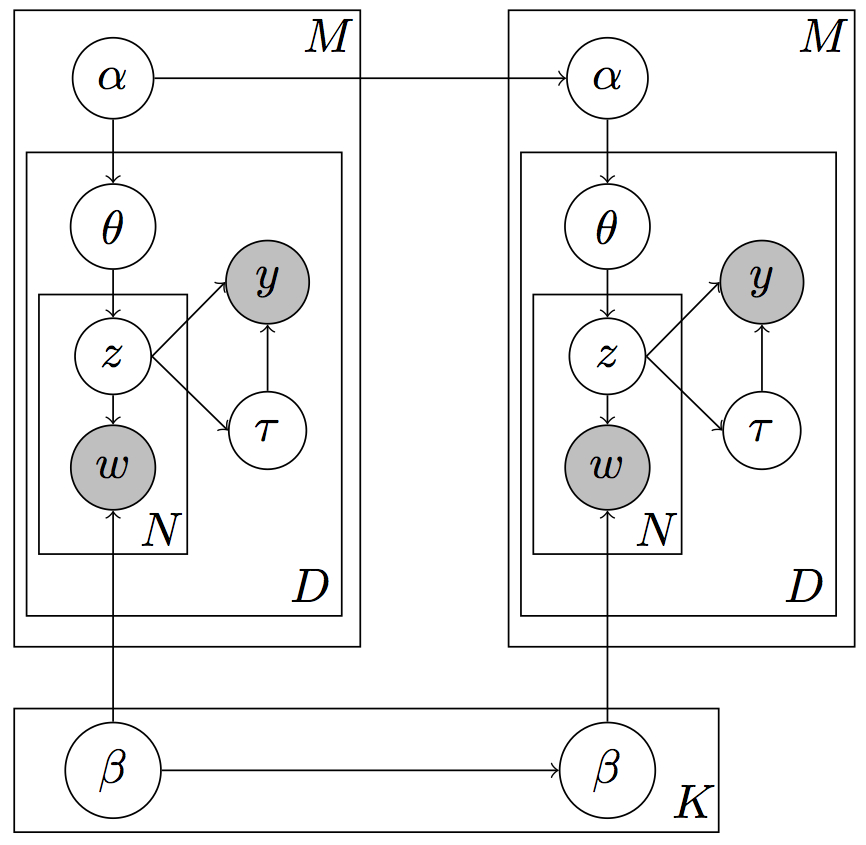
\includegraphics[scale=.25]{plates}
\vspace{-.4cm}
\begin{center}
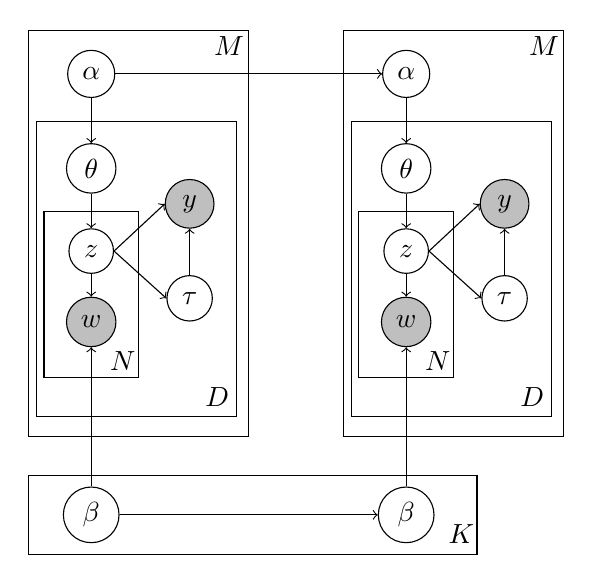
\begin{tikzpicture}

%%%%%% Time 1 %%%%%%%

\node (theta) at (0,.4) [circle, draw] {$\theta$};
\node (z) at (0,-.65) [circle, draw] {$z$};
\node (y) at (1.25,-.05) [circle, draw,fill=lightgray] {$y$};
\node (tau) at (1.25,.-1.25) [circle, draw] {$\tau$};
\node (w) at (0,-1.55)  [circle, draw,fill=lightgray] {$w$};
\node (alpha) at (0,1.6) [circle, draw] {$\alpha$};
\node (b) at (0,-4) [circle, draw] {$\beta$};

\draw[->] (alpha) -- (theta);
\draw[->] (b.north) -- (w.south);

\draw[->] (theta.south) -- (z.north);
\draw[->] (z.south) -- (w.north);
\draw[->] (z.east) -- (y.west);
\draw[->] (z.east) -- (tau.west);
\draw[->] (tau.north) -- (y.south);

\draw (-.8,-3) rectangle (2,2.15);
\draw (-.7,-2.75) rectangle (1.85,1);
\draw (-.6,-2.25) rectangle (.6,-.15);


\node at (1.6,-2.5) {$D$};
\node at (.4,-2.05){$N$};
\node at (1.75,1.95){$M$};

%%%%%% Time 2 %%%%%%%

\node (theta1) at (0+4,.4) [circle, draw] {$\theta$};
\node (z1) at (0+4,-.65) [circle, draw] {$z$};
\node (y1) at (1.25+4,-.05) [circle, draw,fill=lightgray] {$y$};
\node (tau1) at (1.25+4,.-1.25) [circle, draw] {$\tau$};
\node (w1) at (0+4,-1.55)  [circle, draw,fill=lightgray] {$w$};
\node (alpha1) at (0+4,1.6) [circle, draw] {$\alpha$};
\node (b1) at (0+4,-4) [circle, draw] {$\beta$};

\draw[->] (alpha1) -- (theta1);
\draw[->] (b1.north) -- (w1.south);

\draw[->] (theta1.south) -- (z1.north);
\draw[->] (z1.south) -- (w1.north);
\draw[->] (z1.east) -- (y1.west);
\draw[->] (z1.east) -- (tau1.west);
\draw[->] (tau1.north) -- (y1.south);

\draw (-.8+4,-3) rectangle (2+4,2.15);
\draw (-.7+4,-2.75) rectangle (1.85+4,1);
\draw (-.6+4,-2.25) rectangle (.6+4,-.15);


\node at (1.6+4,-2.5) {$D$};
\node at (.4+4,-2.05){$N$};
\node at (1.75+4,1.95){$M$};

%%%%% Tying Together %%%%%
\draw[->] (alpha) -- (alpha1);
\draw[->] (b) -- (b1);

\draw (-.8,-4.5) rectangle (.9+4,-3.5);
\node at (.7+4,-4.25){$K$};

\end{tikzpicture}
\end{center}
\vspace{-.3cm}
\caption{Graphical representation of a dynamic multi-corpus model of text ($w$) and context ($y$) over two time periods. Each topic's natural parameters ($\beta$) evolve over time. The logistic normal determinants of topic proportions ($\alpha$) co-evolve across the $M$ domains.}
\vspace{-.5cm}

\label{plates}
~\\~\\

{\bf Generative Process}
\begin{enumerate}
\item Draw $\alpha_t | \alpha_{t-1} \sim  \mathcal{N}(\mu_t,\sigma^2I)$
\item Draw topics $\beta_t|\beta_{t-1}\sim \mathcal{N}\left(\beta_{t-1},\delta^2I \right)$
\item For each domain $m$:
\begin{enumerate}[a.]
\item For each document in $m$:
\begin{enumerate}[I.]
\item  Draw $\eta \sim \mathcal{N}\left(\alpha_{m,t},a^2I \right)$
\item For each word:
\begin{enumerate}[i.]
\item Draw $Z \sim \text{Mult}(\pi(\eta))$
\item Draw $W \sim \text{Mult}(\pi(\beta_{t,z}))$
\end{enumerate}


\end{enumerate}
\end{enumerate}
\end{enumerate}

\vspace{-1.6cm}
\end{wrapfigure}

Another important feature of our framework is that each
domain-specific model family incorporates an integrated probabilistic
representation of domain-specific metadata describing the
organizational structural context ($y$) and a generic metadata
$\tau$. Generally, $\tau$ will be topic-dependent (e.g.,
topic-specific network structure, as in our pilot work); however, in
figure~\ref{plates} we leave these two components without complete
specification, since the structure and parameterization
will vary considerably over the $M$ domains, as described below.

Although we will likely need to adapt this integrated modeling
framework for each government organization, we anticipate that that
the key properties of the generative process will be similar to those
summarized in figure~\ref{plates}.


%We will derive models with a common set of topics across domains, but varying attention to topics in each domain. The attention to each topic will be given by a logistic transformation of Gaussian-distributed attention parameters. For each topic $t$, there will be four domain-specific attentiveness parameters. The four Gaussian attention parameters will be modeled as a vector autoregression \cite{Banbura2010}. This will permit topics to be related across domains. Thus, the attention level to a topic in each domain will be related to the attention level to a topic in every other domain, up to a selected number of periods into the past.


%A vector autoregression model is a classic linear regression model for time serial data. The estimated parameters of the vector autoregression model will be assessed in order to understand relationships across domains. This is a highly flexible framework for integrating domain-specific models. It works whenever a common set of topics is used to model the dynamic corpora across domains. Thus, this approach permits flexibility in tuning or possibly changing the form of the domain-specific models proposed above. Another major advantage of the vector autoregressive framework is that it constitutes an effective predictive forecasting model \cite{Banbura2010}. This would permit a forecast of, e.g., legislative attention to an issue in the future given current and past legislative, informal intra-governmental and outside input attention to an issue.



\subsection{Modeling Outside Input}

\noindent {\bf Data description:} To define a model for citizen input it is important to first identify the form of the data we will gather on citizen input. Via public records requests, we will collect all emails sent to county government officials by those outside of government. Though some government organizations have experimented with different electronic input modes, the email message is still the workhorse of direct advocacy {\bf cite}. We actually do not need to submit a separate request for this data, as they come with the in and out-boxes of government officials.

~\\
\noindent {\bf Model description:} We will model citizen input by
developing a new dynamic cluster--recipient topic model. This model
will draw upon ideas from dynamic topic modeling \cite{Blei2006}, as
well as previous work on modeling email \cite{McCallum2005}, including
our pilot research \cite{Krafft2012}. McCallum et al.'s
author--recipient topic model learns shared topics for the entire
corpus as well as different levels of attention to each topic for each
author--recipient pair \cite{McCallum2005}. For our data, learning
specific author--recipient distributions is not appropriate as many of
the authors of outside input messages will send only a handful of
emails. It will therefore be advantageous to aggregate over several
like-minded authors. We will group outside contacts into clusters such
that each author belongs to one of the clusters with some probability
(i.e., a mixture model) and each cluster is attentive to each topic
with varying degrees. We intend to use nonparametric Bayesian
clustering methods, which obviate the need to select the number of
clusters a priori. PI Wallach has significant expertise in this
area~\cite{Wallach2008,Wallach2010}. Within the domain of governance,
this clustering approach maps very well onto the concept of partisan
factions~\cite{}. The dynamic properties of the model will be handled using a
logistic--normal model of topic dynamics \cite{Blei2006}. This
approach will permit us to understand (1) the overall content of
citizen input, (2) source-specific peculiarities in the content of
input, (3) recipient-specific peculiarities of input content and (4)
the over-time change in the content of input.

~\\
\noindent {\bf Computer science contribution:} The primary computer
science contribution offered by work on this model will be the
development of a new Bayesian latent variable framework for modeling
directed communications (described above) and associated inference
algorithms. This framework is related to both the author--recipient
topic model and to Grimmer et al.'s work on modeling representational
style. This multifaceted focus provides a coherent approach for
dealing with author sparsity and identifying like-minded authors.

~\\
\noindent {\bf Political Science contribution:} The primary political science contribution offered by the application of this model will be an analysis of issue (i.e., topic) factions. This will offer a partition of authors that is very consistent with the concepts of partisan faction. Moreover, this analysis will set the framework for differentiating the influence of different factions of authors on the legislative agenda.

\subsection{Modeling Informal intra-governmental Communications}

\noindent {\bf Data description:} The data for informal
intra-governmental communications will also utilize the email data
collected through public records requests. Since we will have all
email for the officials, we will be able to model the complete
communication network over time.

~\\
\noindent {\bf Model description:} In this phase, we will make the
most explicit use of the team's pilot research. We will develop a new
dynamic topic-specific model of communication networks, in which the
networks are projected in to Euclidean spaces to facilitate
visualization and exploration. The topic dynamics will again be
modeled using a logistic-normal specification. This characterization
will permit us to understand how the content and network context of
intra-governmental communications evolve. Figure
\ref{Figure:LatentSpace} illustrates the results from our pilot
topic-partitioned communication network analysis. The dataset under
analysis is a corpus of all emails among department managers from New
Hanover County, North Carolina in the month of February, 2011. These
are four selected topic-network-spaces. The word types listed at the
top of the plots are the five most likely for the respective
topic. Nodes are placed closer together in the inferred latent space
if they are more likely to exchange emails on the respective
topic. This modeling approach provides estimates that permit intuitive
exploration of the structure of a communication network within a given
topic.

~\\
\noindent {\bf Computer science contribution:} The primary computer
science contribution offered by this component is the development of a
new dynamic model (and associated inference algorithm) that builds
upon the model developed by the PIs in their pilot research
\cite{Krafft2012} to a dynamic context. We will extend this model to
incorporate over-time (Markov) drift in the vertices' positions in the
latent space \cite{Sarkar2005}, which will enable us to forecast
evolution in communication network structure.

~\\
\noindent {\bf Political Science contribution:} The primary political science contribution offered by the application of this model will be an analysis of how government communication network structure and the content of communications co-evolve. This will provide an opportunity to understand when, in the lifecycle of topic attention, network structure changes. Given the literature on the optimal configuration of communication networks \cite{Mason2008,Mason2012}, these results will permit us to assess how long it takes  a government communication network structure around a given topic to configure into an efficient network.




\subsection{Modeling Formal intra-governmental Communications}

\noindent {\bf Data description:}  Policy development that takes place at the county level occurs within county legislatures. Digitized archives of legislative meeting minutes are typically (indeed in every locality that we have checked) available on the web, but are certainly accessible via public records requests. This data will offer a window into whether issues that are being communicated to the government from outside actors and/or topics that arise through informal intra-governmental communications make their way to the legislative agenda.

~\\
\noindent {\bf Model description:} Our modeling approach with regard to legislative meeting minutes is informed by the political science literature on decision-making in legislatures. Most of this research focuses on the process of coalition-building in legislative processes \cite{Aldrich1995}. Since the vast majority of legislatures require majority support to establish policy, the primary task of a legislator is to lobby, placate and persuade his or her colleagues regarding proposed legislation. The coalition-building process gives rise to factionalism, which induces high positive association between the priorities of those in the same faction and high negative association between the priorities of those in different factions.

We will develop new statistical topic models that build upon the
correlated topic model \cite{Blei2005} and the author--topic model
\cite{Steyvers2004} in order to take advantage of the multiple-meeting
structure of the data to assess the associations underlying the
generation of meeting proceedings. Like the author--topic model, there
will be a common set of topics discussed by all legislators at a given
point in time, but proportional attention to topics will vary across
legislators. The seminal correlated topic model embeds a correlation
structure among topics. We will instead examine correlation between
legislators' attention to topics. Specifically, we will parse each
meeting into statements made by each county legislator. Then, we will
fit a logistic--normal parameterization of the author--topic model that
estimates a covariance matrix over legislators regarding their
attention to topics in each meeting. This will capture the varying
priorities among legislators and the correlations among them that
arise through the legislative bargaining process.

~\\
\noindent {\bf Computer science contribution:} The primary computer
science contribution offered by work on this model will be the
development of a statistical topic model (and associated inference
algorithm) that incorporates interdependence among authors. This will
constitute an indispensable component of our input-response-feedback
modeling, but would also be independently applicable to countless
real-world contexts involving contemporaneous text generated by the
same authors over many instances in time (e.g., any sort of meeting
for which the minutes are recorded).

~\\
\noindent {\bf Political Science contribution:} The primary political science contribution offered by the application of this model will be an analysis of how interdependence manifests in legislative deliberation. We will be able to answer such questions as:
\begin{itemize}
\item Do legislators of the same political party focus on the same issues in legislative deliberations?
\item Do legislators of the same gender and/or ethnicity focus on the same issues in legislative deliberations?
\end{itemize}


\subsection{Modeling Legislative Output}


\noindent {\bf Data description:}  We will gather data on the statutes created by each county in order to examine implementation of topics that arise in the public, informal intra-governmental communications, and on the legislative agenda. These data are available on the web for most counties, and are certainly a matter of public record and would be available upon request. For some counties, it is straightforward to extract how legislators voted on a measure from the meeting minutes. For other counties, however, this is not as simple and may not be feasible.

~\\
\noindent {\bf Model description:} Regardless of whether we can
extract votes on legislation, we will use a dynamic topic model with a
logistic--normal autocorrelation structure to model the content of
legislation. If the votes are available, we will augment the dynamic
topic model with a topic-specific network structure. The network will,
however, take on a different form. The fully-visible Boltzmann Machine
constitutes a probability model of jointly observed binary switches
that is parameterized to model the tendency for each switch to be 'on'
as well as the pairwise association between the states of each dyad of
switches \cite{Gunawardana2008}. This can be used to model binary
votes with voters akin to switches, as illustrated by work co-authored
by PI Desmarais that analyzes voting on the US Supreme Court
\cite{Desmarais2010}. This will allow us to jointly model the
attention to topics in legislation as well as the associations among
legislators' final votes on policy. Figure \ref{Figure:boltz}
illustrates the results from applying a fully visible Boltzmann
machine to vote data. Specifically, the data modeled are the votes of
the nine justices in each US Supreme Court case from the 2007 and 2008
terms. The data are coded as 0 for a conservative vote and 1 for a
liberal vote. Panel (a) gives the estimated tendencies of each justice
to vote liberal and panel (b) depicts the strong positive and negative
associations between justices. The Boltzmann machine offers a powerful
approach to representing the individual and interactive tendencies
among a group of decision-makers.

~\\
\noindent {\bf Computer science contribution:} The primary computer
science contribution offered by work on this topic is the development
of a statistical model that simultaneously models the content of a
document annotated with a vector of choices. This model will be
applicable to any context in which there is voting on a policy
documented in text.

~\\
\noindent {\bf Political Science contribution:} This model will enable us to assess the likely degree of agreement among legislators surrounding legislation -- using topic-specific Boltzmann machines -- at any point in time. The primary political science contribution offered by the application of this model will be an analysis of how topics and agreement surrounding topics co-evolve. Of high specific interest will be whether attention to legislation is associated with the degree of agreement among legislators on a given topic.




\subsection{Overall Project Outputs}

Each of the modeling phases described above constitutes a novel contribution to the literature on natural language processing. The four domain-specific models have not appeared in the literature in their proposed form. Each would therefore constitute a publishable innovation that might appear in such venues as NIPS, AISTAT, and ICML. Of course, decisions about whether to include multiple innovations in the same discrete papers will depend upon the results of empirical experiments, overlap in inferential strategies and several other factors that cannot be perfectly anticipated at this point.

Another, particularly notable, machine learning contribution of this project will be the development of our vector autoregressive framework for building multi-corpora dynamic models of text and context. The framework will be motivated with the problem of modeling organizational responsiveness to outside input and illustrated through the combination of our domain-specific models to model the input-response-feedback cycle in local governments. This will constitute standalone research that is publishable in high profile machine learning conferences.

The major social scientific contributions will come in the form of several analyses of how the sociopolitical contexts and textual content co-evolve. The domain-specific models will individually provide for important innovations in our understanding of government and local government processes. For instance, the analysis of email networks will permit us to assess whether government communication networks are structured to effectively solve problems. As a second example, the legislative meeting minute models will be useful in assessing whether political discussion is as factional at the local level as it is in the US Congress \cite{}. The biggest contribution to political science offered by this project will be the analysis of the cross-domain relationships inferred using the vector autoregressive logistic-normal model. We will be able to speak in precise detail to a fundamental question of growing important to political scientists and practitioners alike -- how do governments respond to open outside input?

\begin{figure}
\begin{center}
{\bf Alachua County, Florida} \\
 {\bf url:} \texttt{http://www.alachuacounty.us/Depts/BOCC/Pages/CommissionerEmailArchive.aspx} \\
 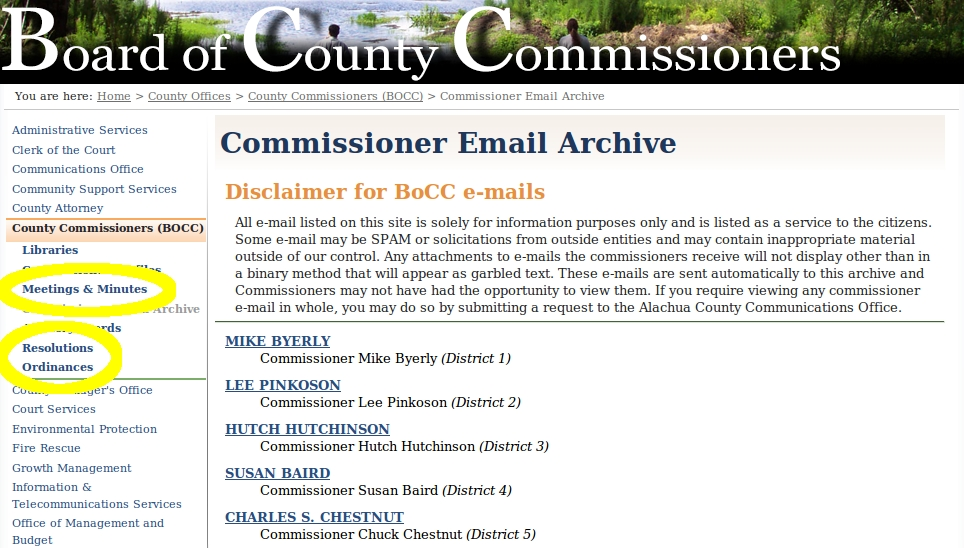
\includegraphics[scale=.45]{AlachuaBOCC.jpg} \\~\\
 {\bf Corvallis, Oregon} \\
 {\bf url:} \texttt{http://www.corvallisoregon.gov/index.aspx?page=65} \\
  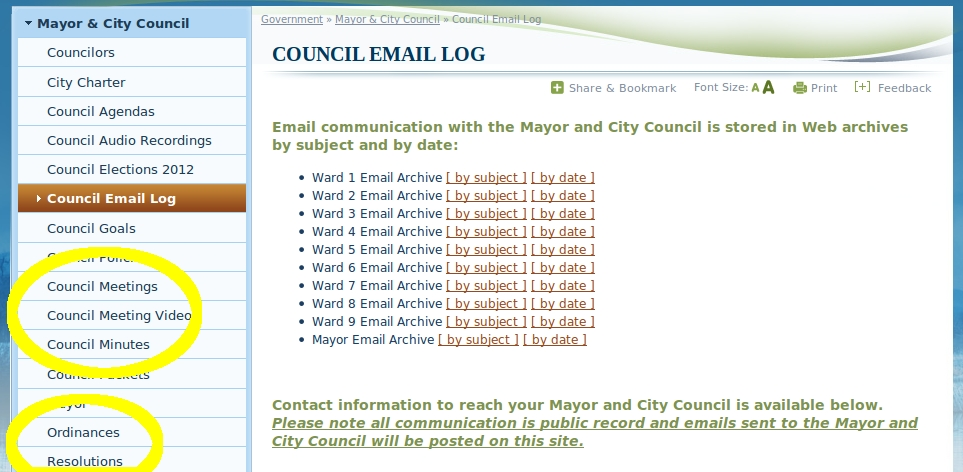
\includegraphics[scale=.45]{CorvallisOR.jpg}
\end{center}
\caption{Web Interfaces to local government email archives. Links to legislative deliberations (i.e., meeting minutes) and legislative outputs (i.e., ordinances and resolutions) are circled in yellow.}
\end{figure}


\subsection{Robustness of Data Collection Plan}

One encouraging aspect of our proposed project is that the data collection is highly scalable and adaptable, but we are more than assured to have access to several government data sources. As proposed, we will lean heavily on public records requests in an ambitious effort to gather data from hundreds or even thousands of localities. This broad coverage would permit us to derive highly generalizable empirical findings and test our statistical models on governments that vary in structure, region, population size and several other demographics. In our experience during the pilot data collection phase, local governments have been more than happy to comply with our requests.

However unlikely, it is certainly within the realm of possibility that the demeanor of local governments toward large scale public records requests will change course. If this happens, we will still be able to gather more than enough data to carry out the project. This is because for many localities, including several counties in Florida and cities in North Carolina, California and Oregon, all of the communication records that are required for our research are available on government websites. These sources include emails to and between government officials, minutes of legislative meetings, and records of adopted policies. Figure \ref{screens} illustrates the web interfaces to this data for two such localities, Alachua County, Florida and the City of Corvallis Oregon. As can be seen from these intuitive and open web interfaces, ample data required to model the interrelationships among domain-specific corpora are readily available.





\section{Timeline and Division of Labor}

We propose to complete this research within a period of three years. The four major tasks will be (1) development and implementation of new statistical models, (2) data collection and cleaning, (3) application of methods and assessment on empirical data, (4) social scientific analysis of results. We divide the project period into quarters and in Table 1, we provide a breakdown of the primary activities of the project, along with an assessment of when the tasks will be completed.


\begin{table}[h]
\caption{Schedule of Project Activities}
\begin{center}
\begin{tabular}{|l|l|l|l|}
\hline
{\bf Lead PI} & {\bf Activity} & {\bf Period} \\ \hline
Wallach & domain-specific model derivation   &   Q1-- Q8 \\
& and implementation &  \\ \hline
Desmarais & data collection (e.g., public records requests  & Q1-- Q3 \\
&  and web-scraping)  and organization & \\ \hline
Wallach & experimentation and assesment with county & Q4 -- Q8 \\
&  government data & \\ \hline
Desmarais & social scientific analysis  of & Q5 -- Q8 \\
& domain-specific results & \\ \hline
Wallach & development and application of integrated & Q6 -- Q12 \\
& vector autoregressive logistic normal model & \\ \hline
Desmarais & social scientific analysis of integrated & Q9 -- Q12 \\
& vector autoregressive logistic normal model & \\ \hline

\end{tabular}
\end{center}
\label{schedule}
\end{table}%



\section{Broader Impacts}

The proposed project will offer broad impacts that advance the core societal mission of the Information Integration and Informatics (III) program, directly enhance educational offerings at the University of Massachusetts and elsewhere and provide valuable interdisciplinary training opportunities related to an emerging area of research -- computational social science.

\subsection{Societal Mission}

The III program supports the development of computational tools and analytical approaches that enable the massive, diverse and complex streams of data to be efficiently utilized to produce scientific, technical and societal advances. Our proposed research addresses this mission, precisely. We will develop methods that enable organizations to assess their responsiveness to electronic open outside input using corpora of data that are already archived for other purposes (e.g., electronic messages, formal meeting records, distinct policy outputs). Also, on the more precise subject-matter of government responsiveness to outside input, we will assess the evidence for the effectiveness of 'we-government' style citizen contributions to the policymaking debate. In sum, this project will (1) offer computational tools that enhance the ability of organizations to remain responsiveness to outside input, (2) leverage large data archives already collected by countless organizations and (3) offer a critical assessment of a major new area of technological innovation for government.

\subsection{Education and Training}

Both PIs are strongly committed to bringing their research into the classroom. PI Wallach regularly teaches a graduate seminar titled, 'Computational Social Science' in which state-of-the art innovations in computational social science are studied at-length. The results of the proposed project would certainly be integrated into the curriculum. PI Desmarais teaches graduate courses in network analysis at the University of Massachusetts and the University of Michigan (summer program). These courses integrate up-to-date methodological innovations in his research. The course material will be updated to reflect the contributions of the proposed project. PI Desmarais has also contributed to the NSF-supported Online Portal for Social Science Education in Methodology (OPOSSEM) - an open source online archive of methodological instructional materials. Instructional materials related to the current project would be posted to OPOSSEM.

The proposed project will support a graduate student in computer science and one in political science at the University of Massachusetts, as well as several undergraduate research assistants.  The proposed research represents a genuinely interdisciplinary research program in the emerging field of computational social science. Long-term focused training for graduate students will provide valuable research experience and socialization on interdisciplinary projects - a growing focus of the scientific community. Undergraduate RAs will also gain valuable complimentary experiences. Computer science students will have the opportunity to work on technical problems that address highly important sociopolitical problems, and political science students will be directly exposed to the ways in which technical analysis and innovation can enhance knowledge of the public policy process. Encouraging sincere interdisciplinary engagement is a central mission at UMass Amherst, signified by the establishment and growing prominence of the UMass Computational Social Science Initiative (cssi.umass.edu). Support of the current project will provide an important opportunity for graduate students to engage in a multi-year cross-disciplinary collaborative project.

\subsection{Broadening Participation of Underrepresented Groups}

Both PIs Wallach and Desmarais have records of making concerted
efforts to broaden the participation of underrepresented groups. PI
Wallach co-founded the Women in Machine Learning Workshop -- an
ongoing annual meeting (and associated executive board) of scholars
that bolsters the small network of female researchers in machine
learning. In 2011, preceding the NSF-sponsored `Visions in
Methodology' conference for women in political methodology at The Ohio
State University, PI Desmarais offered a one day workshop on
statistical inference with network data (featuring the methods he has
developed and applied in his research). Given the results of the
proposed projects, both PIs will continue to pursue training
opportunities that focus on underrepresented groups.



\section{Results From Prior NSF Support}

% 5 pages or fewer of the 15 pages for entire description document.
% include results from NSF grants received in the past 5 years.
% if supported by more than one grant, choose the most relevant one
% for each grant, include: NSF award number, amount, dates of
% support, and publications resulting from this research.
% due to space limitations, it is often advisable to use citations rather
% than putting the titles of the publications in the body
% of this section

% e.g.: "My prior grant, "Uses of Coffee in Mathematical Research" (DMS-0123456,
% $100,000, 2005-2008), resulted in 3 papers [1],[2],[3], demonstrating..."

% if requesting postdoctoral research salary, a supplemental 1-page document
% called "Postdoc Mentoring Plan" will be require

\begin{comment}

\begin{figure}[h]
\vspace{-.6cm}
\begin{center}
\begin{tabular}{m{2.5in}m{2.5in}}
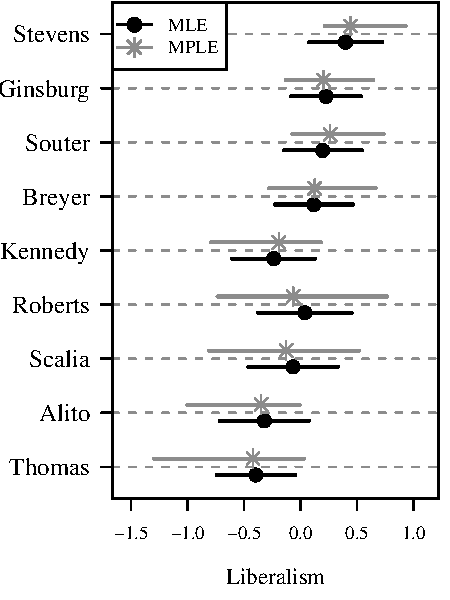
\includegraphics[scale=.65]{fixef} & 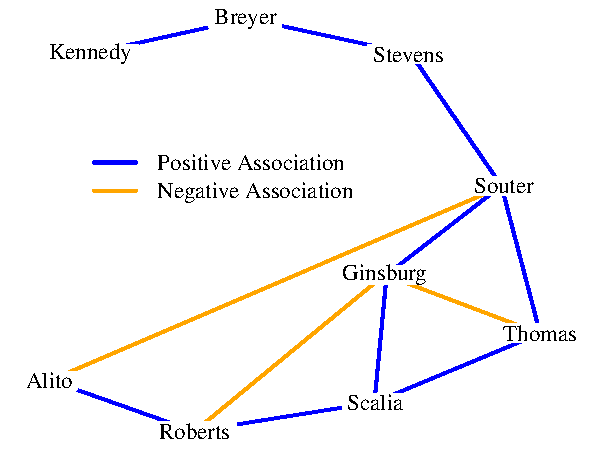
\includegraphics[scale=.75]{infnet}\\
(a) Estimates of Justices' Ideal Points & (b) Significant Associations Between Justices \\
\end{tabular}
\end{center}
\vspace{-.3cm}
\caption{The bars in (a) span 95\% confidence intervals. In (b) an edge is drawn if the association parameter has the respective sign in at least  95\% of the bootstrap samples.}
\label{Figure:boltz}
\end{figure}

\end{comment}




